\documentclass{article}
\usepackage{amsmath}
\usepackage{xcolor}
\usepackage{gensymb}
\usepackage{ragged2e}
\usepackage{graphicx}
\usepackage{gensymb}
\usepackage{mathtools}
\newcommand{\mydet}[1]{\ensuremath{\begin{vmatrix}#1\end{vmatrix}}}
\providecommand{\brak}[1]{\ensuremath{\left(#1\right)}}
\providecommand{\norm}[1]{\left\lVert#1\right\rVert}
\newcommand{\solution}{\noindent \textbf{Solution: }}
\newcommand{\myvec}[1]{\ensuremath{\begin{pmatrix}#1\end{pmatrix}}}
\let\vec\mathbf
\begin{document}
\begin{center}
        \textbf\large{CHAPTER-11 \\ TRIANGLES}
\end{center}
\section{Exercise 11.2}
Q2.Construct a triangle $ABC$ in which $BC=8cm$,$\angle{B}=45^0$ and $AB-AC=3.5cm$. \\
\textbf{Solution:}\\
Let $\vec{A}$,$\vec{B}$ and $\vec{C}$ are the vertices of the triangle with coordinates.
Given $BC=8cm$.So the coordinates of vertices $\vec{B}$,$\vec{C}$ are:
\begin{center}
{
$\vec{B}$ =$\begin{pmatrix}
0 \\
0 
\end{pmatrix}$ 
\vspace{1mm}
$\vec{C}$=$\begin{pmatrix}
8 \\
0
\end{pmatrix}$ 
\vspace{1mm}
}
\end{center}
Also given $\angle{B}=45^0$,so by finding the coordinates of the other side we can form a required triangle. \\
 \vspace{2mm}
 The input parameters for this construction are
 \begin{table}[h]
	  \centering
	  \begin{tabular}{|c|c|c|}
  \hline
  \textbf{Symbol}&\textbf{Value}&\textbf{Description}\\
  \hline
  a & 8cm & BC\\
  \hline
  $\theta$ & $45^0$ & $\angle{BC}$ in $\Delta$ABC \\
  \hline
	k & 3.5 & AB-AC i.e(c-b)\\
  \hline
\end{tabular}

	  \caption{Parameters}
	  \label{tab:Table1}
\end{table}


\raggedright\textbf{Caluclating Other Coordinate: } \\
  \raggedright Let $\vec{A}$ = c
  $\begin{pmatrix} 
 \cos \theta\\
  \sin\theta \\
\end{pmatrix}$ \\
\raggedright Using the Cosine formula in  $\Delta$ABC, \\ \vspace{3mm}
\begin{equation}
{b}^2 = {a}^2 + {c}^2 - 2accos\vec{B}
\end{equation}
\begin{equation}
(b+c)(b-c) = {a}^2- 2accos\vec{B}
\end{equation}
Given
\begin{equation}
        c-b=k
	\end{equation}
  \begin{equation}
        b-c=-k
 \end{equation}\\
Upon Simplifaction we get:- \\
\begin{equation}
(b+c)(-k) = {a}^2- 2accos\vec{B}
\end{equation} \\
\pagebreak
     From equations (4) and (5) , we obtain the matrix equation:- \\ \vspace{3mm}
     \begin{equation}
        \begin{pmatrix}
	   1 & 1  \\	
	   1 & -1    \\
        \end{pmatrix}
        \begin{pmatrix}
            b \\
            c \\
        \end{pmatrix}
           =
           \begin{pmatrix}
		   \frac{-a^2+2accos\vec{B}}{k} \vspace{3mm}\\
            -k \\
        \end{pmatrix}   
\end{equation}	     
        \vspace{5mm}            
   \begin{equation}
        \begin{pmatrix}
            b \\
            c \\
        \end{pmatrix}
           =
	   \frac{1}{2}
           \begin{pmatrix}
            1 & 1 \\
	    1 & -1 \\
        \end{pmatrix}
	\begin{pmatrix}   
	\frac{-a^2+2accos\vec{B}}{k} \vspace{3mm}\\
	-k \\                                
	\end{pmatrix}	
	\end{equation}           
   \\  
   From the above equation \\
\begin{equation}
	c
	=
	\frac{1}{2}
	\vec{e}_2^T
\begin{pmatrix}
   1 & 1  \\
   1 & -1 \\
    \end{pmatrix}  
	\begin{pmatrix} 
        \frac{-a^2+2accos\vec{B}}{k} \vspace{3mm}
 \\
         -k \\
	\end{pmatrix}
    \end{equation} \\
\begin{equation}  
	c    
        =
	\frac{1}{2(1-\frac{acos\vec{B}}{k})}
	 \vec{e}_2^T
 \begin{pmatrix} 
       1 & 1  \\
       1 & -1 \\
     \end{pmatrix}
	\begin{pmatrix}
         \frac{-a^2}{k} \vspace{3mm} \\
         -k \\
	\end{pmatrix}
     \end{equation}\\
  \begin{equation}
          c
	  =
         \frac{1}{2(1-\frac{acos\vec{B}}{k})}
	  \vec{e}_2^T
	  \begin{pmatrix}
	  \frac{-a^2}{k}-k \vspace{3mm} \\
             \frac{-a^2}{k}+k
          \end{pmatrix}
  \end{equation}\\
\begin{equation}
         c
         =
         \frac{1}{2(1-\frac{8cos45^0}{3.5})}
	  \begin{pmatrix}
	   0 & 1
	  \end{pmatrix} 
     \begin{pmatrix}
	  \frac{-64}{3.5}-3.5 \vspace{3mm} \\
	   \frac{-64}{3.5}+3.5 
     \end{pmatrix}
   \end{equation}\\
\begin{align}
	 c
	 =
	 \frac{1}{2\left(\frac{3.5-5.65}{3.5}\right)}
	 \left(\frac{-64+12.25}{3.5}\right) 
     \end{align}\\
     \begin{equation}
	 c = 12
      \end{equation}	     
%\pagebreak
  The vertices of $\Delta$ ABC are \\ \vspace{3mm}
     \raggedright \textbf{A} = 12$\begin{pmatrix}
                 cos 45 \\ 
                 sin 45 \\
              \end{pmatrix}$
              =$\begin{pmatrix}
                 8.48 \\
                 8.48 \\
                 \end{pmatrix}$
                 \vspace{5mm}
              \\ \raggedright  \textbf{B} = $\begin{pmatrix}
                 0\\
                 0\\
              \end{pmatrix}$
              \vspace{5mm}
             \\ \raggedright  \textbf{C} = $\begin{pmatrix}
                  8\\
                  0\\
              \end{pmatrix}$
              \\
	      \vspace{5mm}
\pagebreak	      
\textbf{Construction:}\\
\begin{figure}[h]
 \begin{center}
	 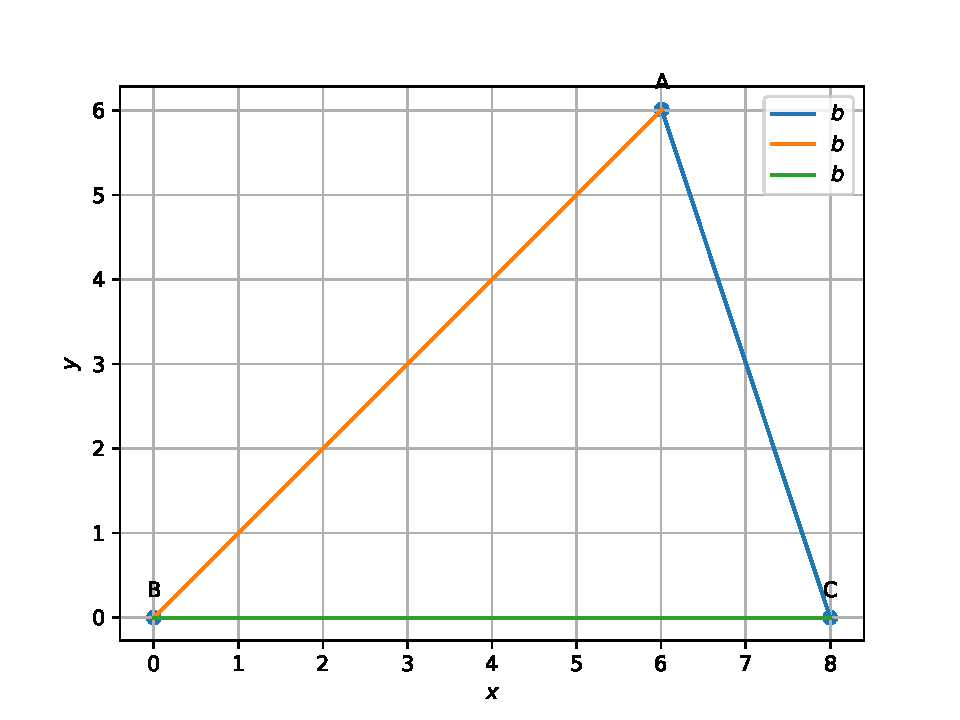
\includegraphics[width=0.5\textwidth]{figs/triangle.pdf}
 \end{center}
 \caption{Triangle ABC}
 \label{fig:Fig1}
\end{figure}	
\end{document}
